\documentclass[a4paper]{article}

%% Language and font encodings
\usepackage[english]{babel}
\usepackage[utf8x]{inputenc}
\usepackage[T1]{fontenc}


%% Sets page size and margins
\usepackage[a4paper,top=3cm,bottom=2cm,left=3cm,right=3cm,marginparwidth=1.75cm]{geometry}

%% Useful packages
\usepackage{amsmath}
\usepackage{graphicx}
\usepackage{caption}
\usepackage{subcaption}
\usepackage{mathptmx}
\usepackage{float}
\usepackage{lmodern} % math, rm, ss, tt
\usepackage[T1]{fontenc}
\usepackage[colorinlistoftodos]{todonotes}
\usepackage[colorlinks=true, allcolors=blue]{hyperref}

\title{Montel for ID20}
\author{Aouadi Yiones}

\begin{document}
\maketitle



\section{Introduction}
With the following document I want to report the results obtained in the simulation of a beam through a Montel system (optical system composed bye two orthogonal mirrors). It has been studied the tolerance in orthogonality using the parameter similar tho those distributed by the AXO DRESDEN Gmbh \cite{greenwade93}

\section{System}

In this simulation was used a Monte-Carlo approach with the following specification

\subsection{Source}

Source parameters
\begin{itemize}
\item Number of rays: $10^6$
\item Source size: 1*1 $\mu $$m^2$
\item Divergence: gaussian profile with a FWHM OF 25$\mu $$rad$ ($\sigma $ = 10.6 $\mu $$rad$)
\end{itemize}
Figure \ref{fig:beam at the source} show the source geometry and  the divergence of the source beam

\begin{figure}[H]
\centering
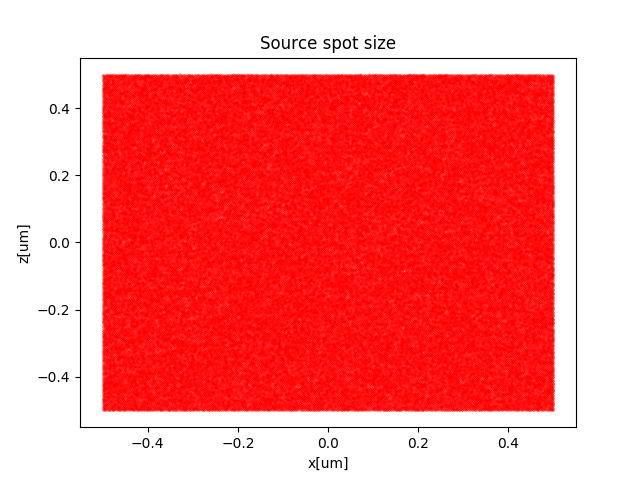
\includegraphics[width=0.495\textwidth]{Spot.png}
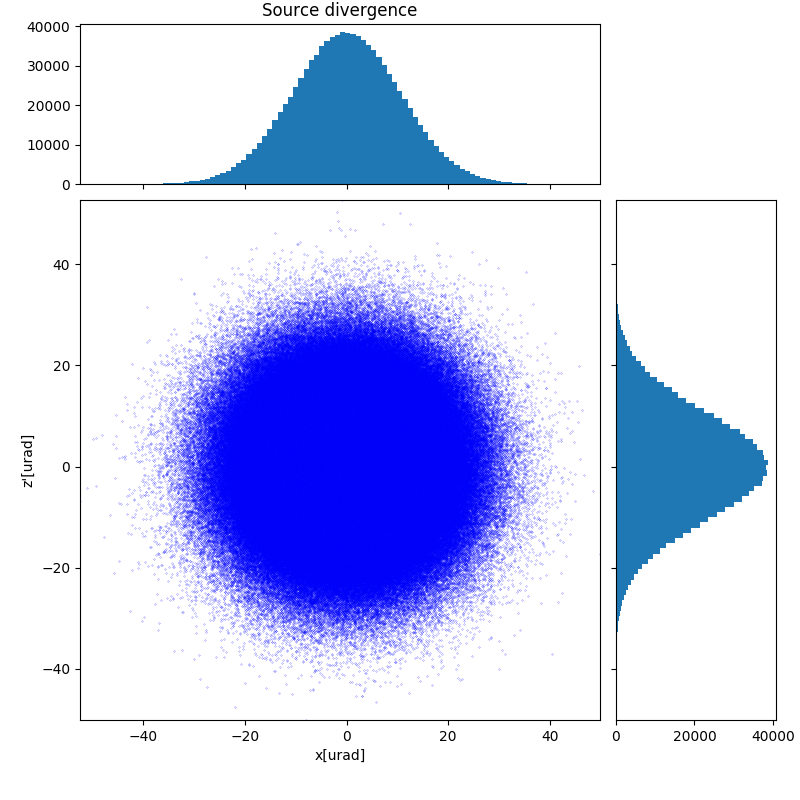
\includegraphics[width=0.495\textwidth]{Initial_divergence.png}
\caption{\label{fig:beam at the source}Source size 1*1 $\mu $$m^2$ }
\end{figure}


\subsection{Montel system}

As mentioned before, two orthogonal mirror (parabolic in this case) were used, with parameters
\begin{itemize}
\item Focal distance (distance between the source and the center of the mirror): f=351$mm$
\item Mirror length: L=300$mm$
\item Mirror width:  W=100$mm$
\item $\Delta$ (error max. between the orthogonal configuration of the two mirrors, negative correspond to have the mirror closer each other, positive further):      $\Delta$ = $\pm$0.03$^{\circ}$
\item Parabola parameter: p=0.23$mm$, that correspond to an incidence angle of 18.1$mrad$ (see appendix A)
\end{itemize}

In figure \ref{fig:Montel system} is showed a 3Dgraphic view of the Montel system with the parameter used. The reference system is solidale with the Montel system, having the $(0,0,0)$ point at the center of the Montel system.


\begin{figure}[H]
\centering
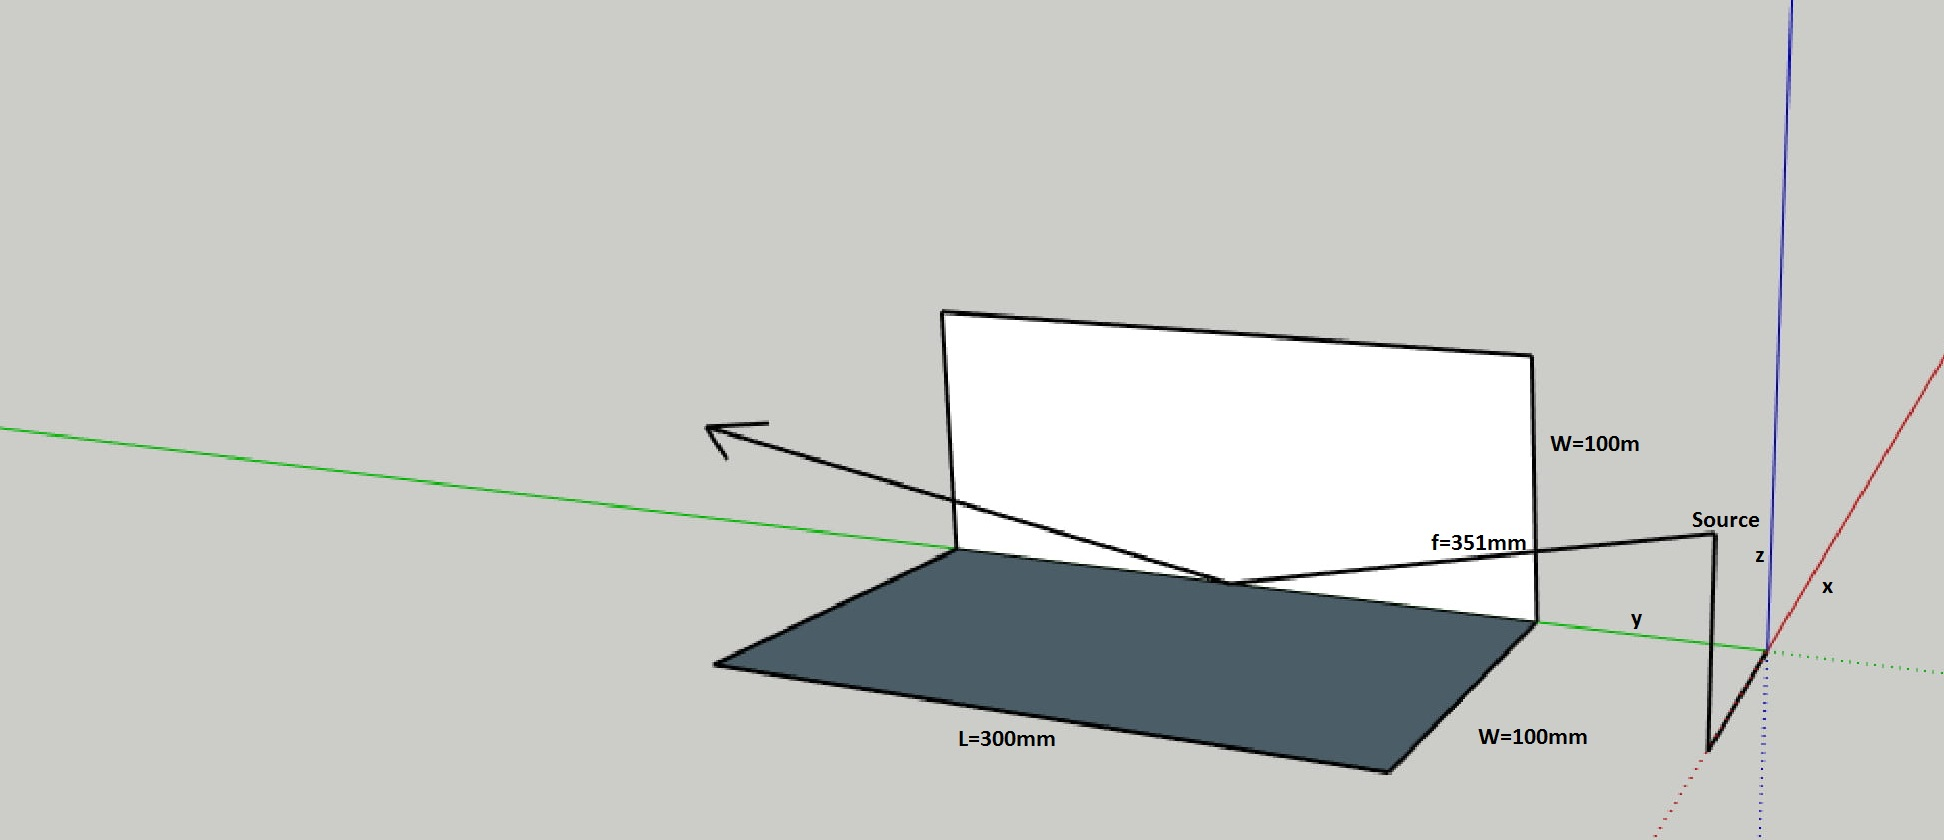
\includegraphics[width=1\textwidth]{MontelSystem.jpg}
\caption{\label{fig:Montel system} Montel system}
\end{figure}

\newpage

\section{Results of beam figure and footprint}

The image plane is positioned at 1$m$ from the center of the Montel system. The property of the beam at the image plane are showed in figure \ref{fig:image}.It is obtained a new spot size with a length of 60$\mu$$m$ in the x direction and 100$\mu$$m$ in the z direction, and the divergence has a dimension  of $\simeq$40$\mu$$rad$


\begin{figure}[H]
\centering
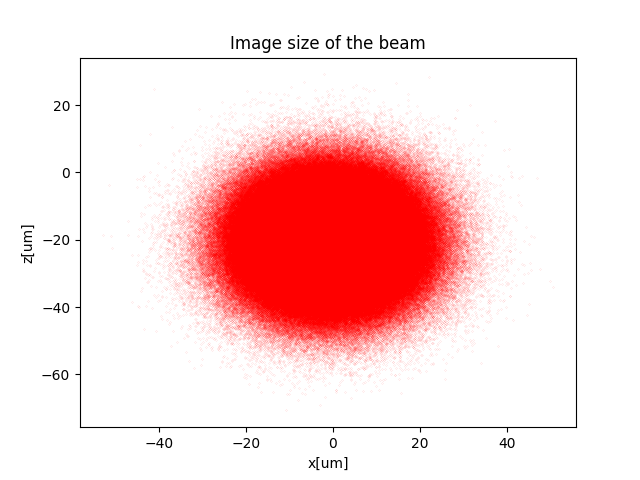
\includegraphics[width=0.495\textwidth]{image_spot.png}
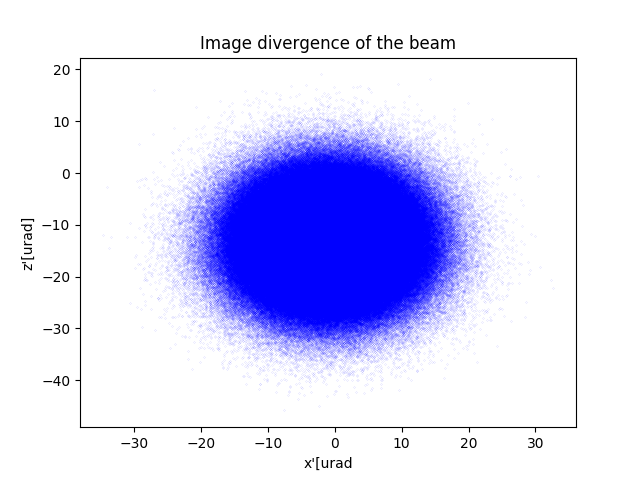
\includegraphics[width=0.495\textwidth]{image_divergence.png}
\caption{\label{fig:image} Left image: size of the beam on the image plane. Right image: divergence at the image plane}
\end{figure}


Moreover is interesting to note the footprint of the two mirror (figure \ref{fig:footprint_oe1}) because the area hit by the beam have a greater component on the y direction (due to the grazing incidence), than in the other direction.The x-length of the xy-mirror, and the z-length of the zy-mirror, is very small (at the order of 20$\mu $$m$) with respect to the y-length that is $\simeq $ 20$mm$

\begin{figure}[H]
\centering
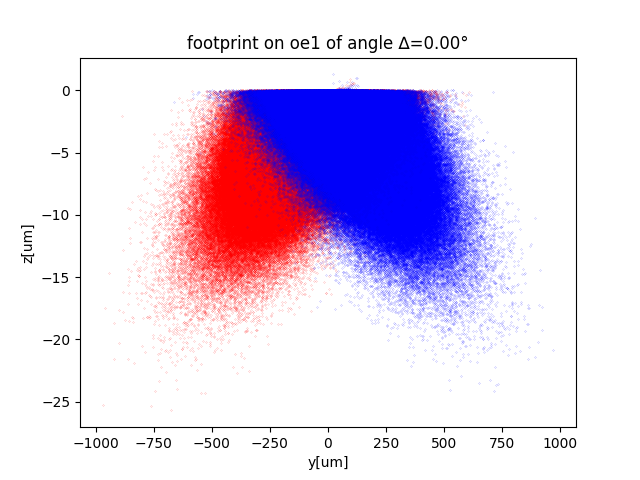
\includegraphics[width=0.495\textwidth]{footprint_oe1.png}
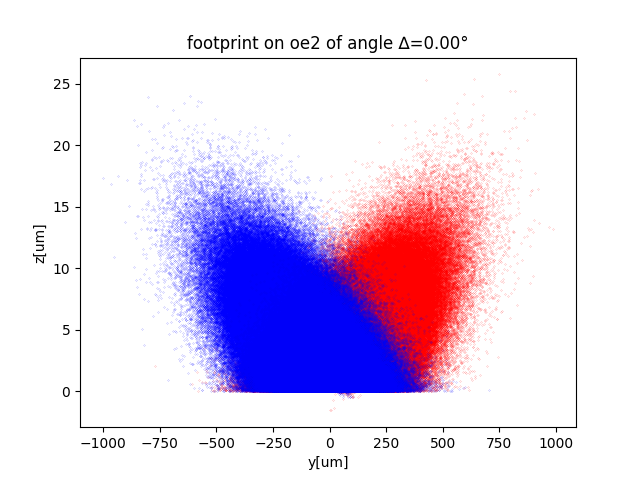
\includegraphics[width=0.495\textwidth]{footprint_oe2.png}
\caption{\label{fig:footprint_oe1} footprint, on the xy-mirror (left figure), zy-mirror (right figure). The red dots are those ray that hit before xy-mirror and after zy-mirror, the blue ones before xy-mirror and after zy-mirror}
\end{figure}

\newpage

\section{Analysis of orthogonality}
Figure \ref{fig:histogram}, \ref{fig:histogram_2} presents the interesting histograms versus the horizontal anlge x' when the angle between the mirrors change ($\alpha $ = 90$^\circ$ + $\Delta$). It can be noted a improvement of the collimation of the beam changing the angle in the case of closer mirrors (delta=-0.01$^\circ$).
\newline Figure \ref{fig:FWHM} show the trend of the FWHM of the x' changing the angle $\Delta$, it is possible to note a minimum for negative angle (this ideal situation is the pink curve reported in figure \ref{fig:histogram}, \ref{fig:histogram_2}) after that the situation become worse. Moreover, the behavior of the FWHM is not symmetrical with respect to 0$^\circ$, in case of negative angle deviation the situation improve for a small range of deviation angle, after that, the trend get worse, on the opposite way, the situation get worse increasing the positive deviation angle.


\begin{figure}[H]
\centering
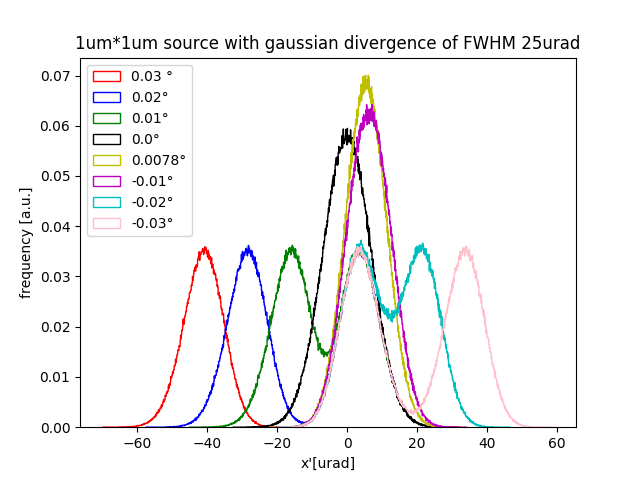
\includegraphics[width=0.68\textwidth]{histogram.png}
\caption{\label{fig:histogram} x' values after the Montel system}
\end{figure}


\begin{figure}[H]
\centering
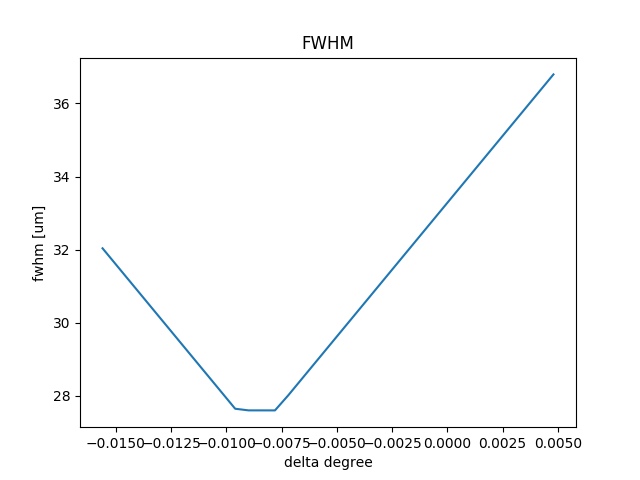
\includegraphics[width=0.68\textwidth]{FWHM.png}
\caption{\label{fig:FWHM} FWHM}
\end{figure}

\begin{figure}[H]
\centering
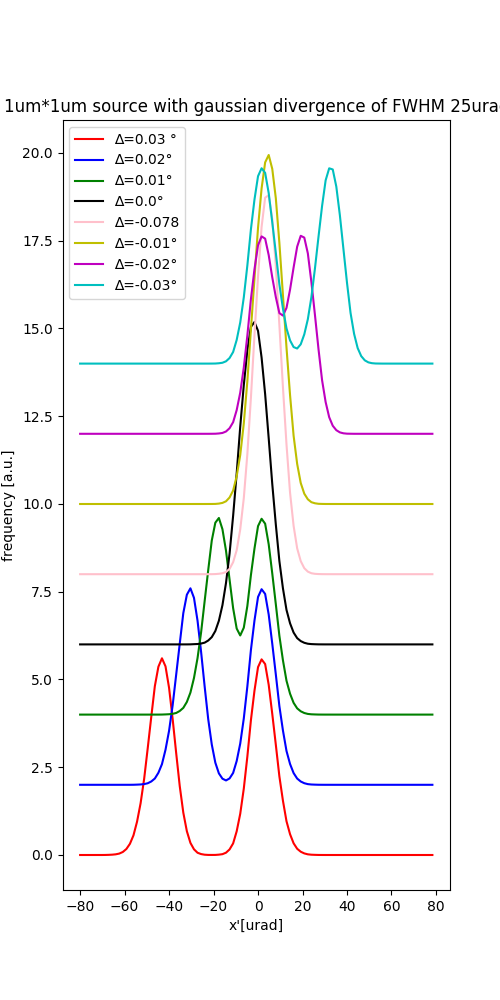
\includegraphics[width=0.8\textwidth]{histogram2.png}
\caption{\label{fig:histogram_2} x' values after the Montel system}
\end{figure}


\section{Best $\Delta$}

In this section is studied how the different source parameter will influence the best value of delta, The simulation are done playing with the source parameter:
\begin{itemize}
\item Source shape: rectangular, circular, gaussian
\item Source dimension
\item Source divergence
\end{itemize}


\begin{table}[ht]
\centering
\begin{tabular}{l|l|l|l|r}
Shape & Dimension  & Divergence [$\mu$rad] & Minimum $\alpha$ [degree] & Min FWHM [$\mu$m]  \\ %<-- an entire row
\hline %<-- the horizontal line
Gaussian & fwhm of 1$\mu$m & 25 & -0.008 & 16.5 \\
Gaussian & fwhm of 1$\mu$m & 250 & -0.1 & 165 \\
Gaussian & fwhm of 1$\mu$m & 2500 & -1 & 1740 \\
Square & side of 1$\mu$m & 25 & -0.009 & 17 \\
Square & side of 1$\mu$m & 250 & -0.1 & 161 \\
Square & side of 1$\mu$m & 2500 & -1 & 1700 \\
Circular & radius of $\frac{1}{\pi}$$\mu$m & 25 & -0.009 & 16.4 \\
Circular & radius of $\frac{1}{\pi}$$\mu$m & 250 & -0.1 & 171 \\
Circular & radius of $\frac{1}{\pi}$$\mu$m & 2500 & -1.35 & 1760 \\


% Note that the LAST row does not need a \\ after it.
\end{tabular}
\caption{Best $\Delta$ value changing the different parameter of the source}
\label{tab:best_delta}
\end{table}

\medskip

Table \ref{tab:best_delta} shows that the source geometry doesn't affects the optimum angle that is ruled by the divergence of the source.


\begin{table}[ht]
\centering
\begin{tabular}{l|l|l|l|r} Spot dimension [$\mu$m$^2$] & Divergence [$\mu$rad] & Minimum $\alpha$ [degree] & Min FWHM [$\mu$m]\\
1*5 & 25 & -7.6 & 16.6\\
2*2.5 & 25 & -7.5 & 16.8\\
3*1.67 & 25 & -7.2 & 16.6\\
4*1.25 & 25 & -8.8 & 18\\
5*1 & 25 & -7.1 & 17\\

\end{tabular}
\caption{Best $\Delta$ value changing the different symmetry of the source}
\label{tab:best_delta_symmetry}
\end{table}


Table \ref{tab:best_delta} shows that the symmetry doesn't affects the optimum angle.

\medskip

\subsection{Best $\Delta$ for a non centered beam}
Here is reported the behavior of the beam when it hit a different point of the Montel system. Table \ref{tab:displacement} is done in this way, the first row and the first coloumn report the point where the beam hit, and, inside the grid, there is the best value of $\Delta$(first row), and the best FWHM(second row).As is showed, the FWHM and the best $\Delta$ is less influenced from the y-position than the others
\newline
Another interesting aspect is that showed in figure , the presence of the second peak decrease with the distance from the y=0 axis position


\begin{table}[H]
\centering
\begin{tabular}{l|l|l|l|l|r}  & y=-1mm & y=-0.5mm & y=0 & y=0.5 & y=1mm\\
\hline
     z     & -0.015$^\circ$ & -0.015$^\circ$ & -0.015$^\circ$ & -0.015$^\circ$ & -0.018$^\circ$ \\
20$\mu$m   & 16.6$\mu$m & 16.5$\mu$m & 16.5$\mu$m & 16.5$\mu$m & 18$\mu$m \\
\hline
     z     & -0.01$^\circ$ & -0.01$^\circ$ &-0.075$^\circ$& -0.005$^\circ$ & -0.01$^\circ$\\
10$\mu$m   & 16$\mu$m & 16$\mu$m & 16$\mu$m & 16$\mu$m &  16$\mu$m  \\
\hline
          & -0.005$^\circ$ & -0.005$^\circ$ & -0.005$^\circ$ & -0.005$^\circ$ & -0.015$^\circ$ \\
          & 14.5$\mu$m & 14.5$\mu$m & 14.5$\mu$m & 14.5$\mu$m & 16.6$\mu$m \\
\hline
     x    & -0.01$^\circ$ & -0.01$^\circ$ & -0.0075$^\circ$ & -0.01$^\circ$ & -0.006$^\circ$ \\
-10$\mu$m & 16$\mu$m & 16$\mu$m & 16$\mu$m & 16$\mu$m & 6$\mu$m \\
\hline
     x    & -0.01$^\circ$ & -0.01$^\circ$ & -0.01$^\circ$ & -0.01$^\circ$ & -0.01$^\circ$ \\
-20$\mu$m & 16.5$\mu$m & 16.5$\mu$m & 16.5$\mu$m $\mu$m & $\mu$m16.5 & 16.5$\mu$m \\

\end{tabular}
\caption{Best FWHM and $\Delta$ for a non centered beam}
\label{tab:displacement}
\end{table}

\begin{figure}[H]
	
    \centering
	\begin{subfigure}{0.4\textwidth}
		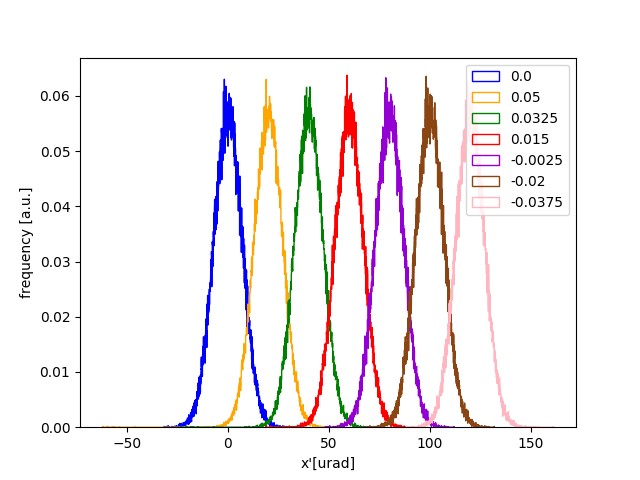
\includegraphics[width=\textwidth]{-20um.png}
		\caption{(-20um,0,0)}
	\end{subfigure}
	\vspace{2em}
	\begin{subfigure}{0.4\textwidth}
		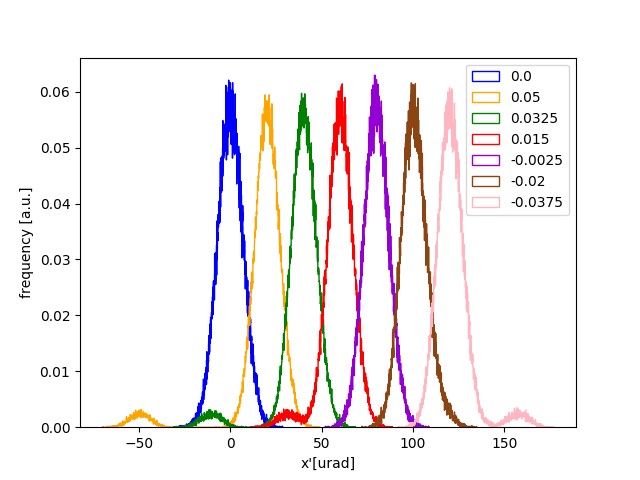
\includegraphics[width=\textwidth]{-10um.png}
        \caption{(-10um,0,0)}
	\end{subfigure}
	\vspace{2em}
	\begin{subfigure}{0.4\textwidth}
		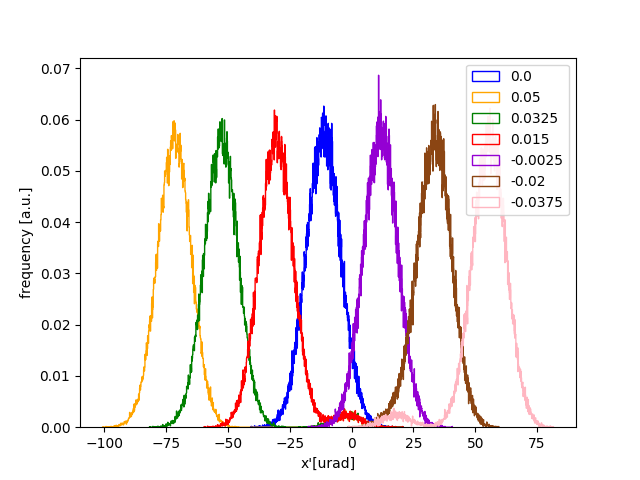
\includegraphics[width=\textwidth]{10um.png}
        \caption{(0,0,10um)}
	\end{subfigure}
	\vspace{2em}
	\begin{subfigure}{0.4\textwidth}
		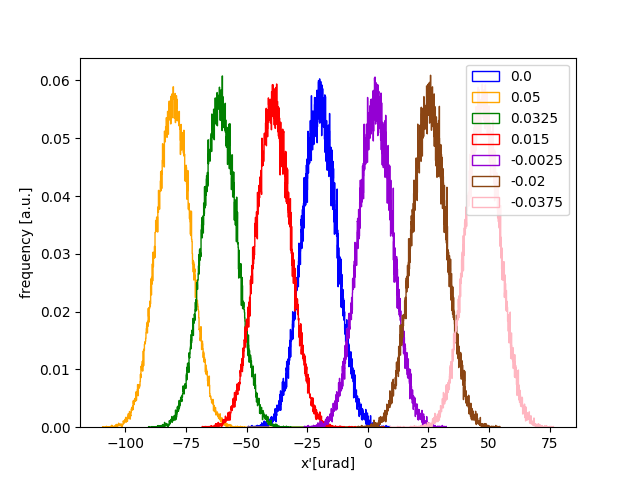
\includegraphics[width=\textwidth]{20um.png}
        \caption{(0,0,20um)}
	\end{subfigure}
	\begin{subfigure}{0.5\textwidth}
    	\centering
		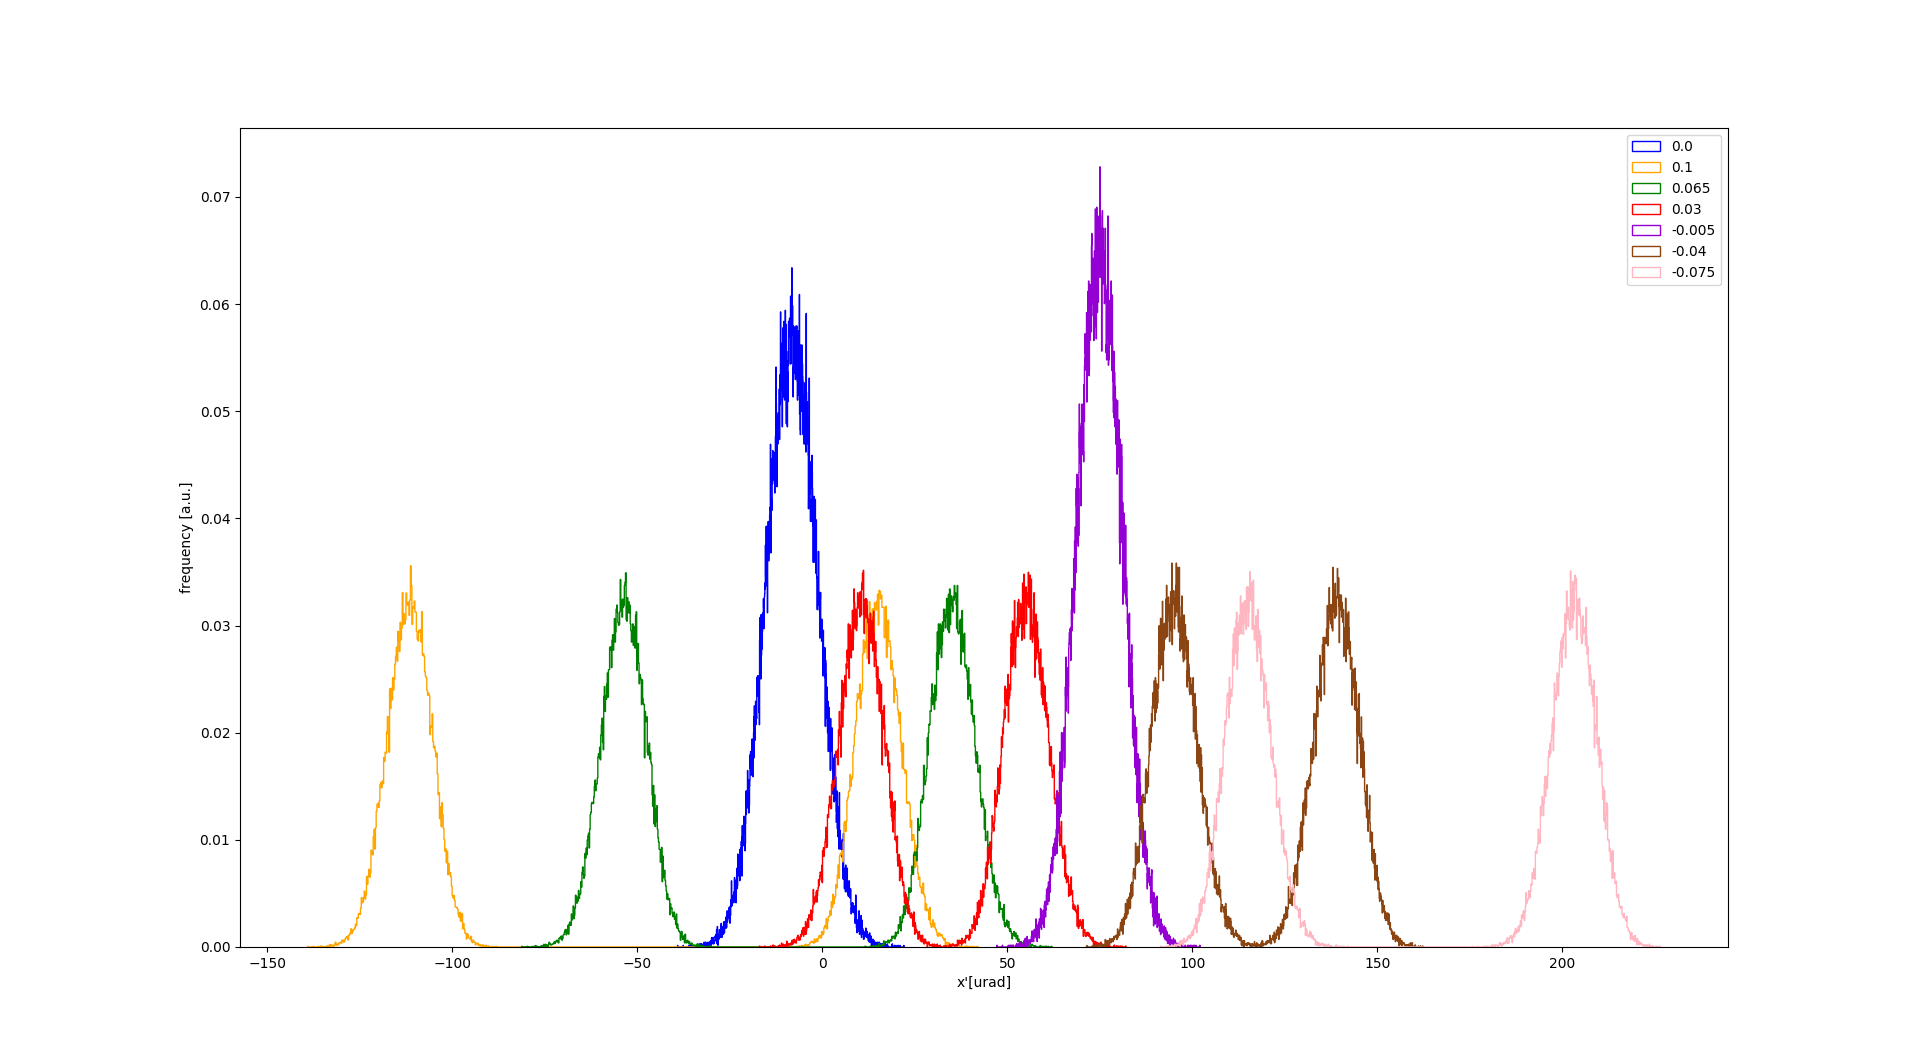
\includegraphics[width=\textwidth]{0.png}
        \caption{(0,0,0)}
	\end{subfigure}
    
    \caption{Beam at the different hitting point (the beam were split on the x-axis)}

\end{figure}


\newpage
\newpage
\appendix{Appendix A: how to find $\theta$}

\begin{figure}[H]
\centering
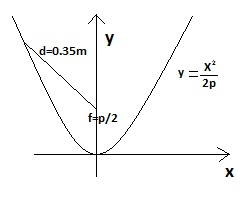
\includegraphics[width=0.6\textwidth]{pparabola.jpg}
\end{figure}

\begin{equation*}
y=\frac{x^2}{2p}
\end{equation*}

\begin{equation*}
d=\sqrt[]{(x_p-x_0)^2+(y_p-y_0)^2}=\sqrt[]{x_p^2+(y_p-\frac{p}{2})^2}
\end{equation*}

\begin{equation*}
x_p=-0.0127046, y_p=0.350885
\end{equation*}

velocity to hit that point starting from $(0, \frac{p}{2})$
\begin{equation*}
v_x=-0.0363024, v_y=0.999341
\end{equation*}

normal at that point
\begin{equation*}
n_x=-0.984005, n_y=-0.17814
\end{equation*}

doing dot product between the normal and the velocity is possible to find
\begin{equation*} 
\theta=arcos(v_x*n_x+v_y*n_y)=88.962^\circ
\end{equation*}

%\cite{baudoin:1998:impara-latex-e-mettilo}

\nocite{*}
\bibliographystyle{alpha}
\bibliography{sample}

\end{document}
